% Auto-generated by r_project/simulation/mc_paper.R
% Generated 2026-11-23 12:34 at commit 9e7ae33 (uncommitted changes)
% Monte Carlo rows: commit(s) 7acc201, 2ae035d, f3382b0, bd2f334, 9ceeb42, c1a3c0b, 94dfe82, f1ebed4, 9e7ae33; targets: commit f3382b0,9ceeb42,c1a3c0b,94dfe82,f1ebed4,bd2f334,9e7ae33,817ab68

\begin{figure}[htbp]
\centering
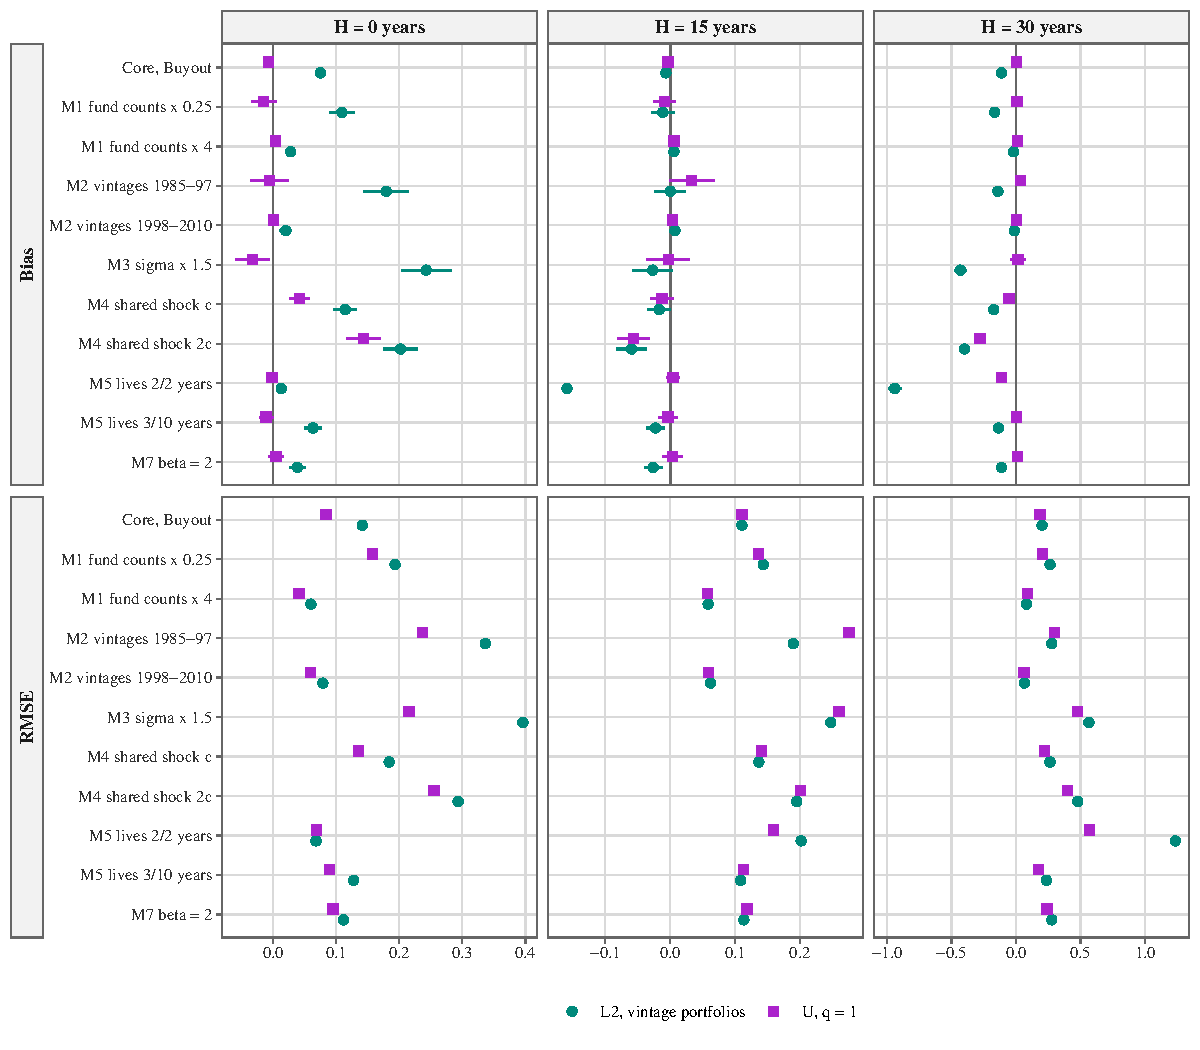
\includegraphics[width=\textwidth]{figure_S2_margins.pdf}
\caption{Monte Carlo: one margin at a time}
\label{fig:mc_margins}
\par\vspace{2pt}
{\scriptsize\textit{Notes:} Bias and RMSE of the single-factor $\hat\beta_{MKT}$ at 0, 15 and 30 years, L2 on vintage portfolios and $U_{v,H}$ with $q_v=1$. Each design changes one feature of the Buyout core (Table~\ref{tab:mc_core}): M1 fund counts scaled by 0.25 (at least 2 per vintage) or 4; M2 the early or late half of the vintage calendar; M3 $1.5\times$ the calibrated $\sigma$; M4 a shared vintage shock of the size that matches the empirical Buyout $U_{v,H}$ level, or twice that (then the $U_{v,H}$ target moves away from the true value, T7); M5 investment and holding periods of 2/2 or 3/10 years; M7 true $\beta_{MKT}=2$. Bars: $\pm2$ Monte Carlo SE of the bias. 250 replications (M5 2/2: 1{,}000).}
\end{figure}
